\documentclass[10pt]{article}
\usepackage[paperwidth=297mm,paperheight=210mm,margin=17mm,headheight=14pt]{geometry}
\usepackage{fontspec}
\setmainfont{Arial}
\setsansfont{Arial}
\usepackage{graphicx}
\usepackage[table]{xcolor}
\usepackage{tikz}
\usepackage{tabularx}
\usepackage{array}
\usepackage{multicol}
\usepackage{fancyhdr}
\usepackage{hyperref}
\usepackage{enumitem}
\usepackage{microtype}
\usepackage{ragged2e}
\definecolor{navy}{HTML}{102B49}
\definecolor{teal}{HTML}{0A9CA8}
\definecolor{mint}{HTML}{DDF6F3}
\definecolor{pale}{HTML}{F3F7FA}
\definecolor{slate}{HTML}{50657A}
\definecolor{line}{HTML}{D7E2E9}
\definecolor{warn}{HTML}{C05445}
\hypersetup{colorlinks=true,linkcolor=teal,urlcolor=teal,pdftitle={ClaimGuard | Phase 1 Architecture and Data Flow},pdfauthor={ClaimGuard Team}}
\setlength{\parindent}{0pt}
\setlength{\parskip}{6pt}
\renewcommand{\arraystretch}{1.28}
\pagestyle{fancy}
\fancyhf{}
\fancyhead[L]{\small\color{slate}CLAIMGUARD \quad / \quad PHASE 1 SYSTEM REPORT}
\fancyhead[R]{\small\color{slate}Architecture and data flow}
\fancyfoot[L]{\small\color{slate}Synthetic claims only \quad | \quad 01 October 2026}
\fancyfoot[R]{\small\color{slate}\thepage}
\renewcommand{\headrulewidth}{0.4pt}
\renewcommand{\footrulewidth}{0pt}
\setlist[itemize]{leftmargin=5mm,itemsep=2pt,topsep=2pt}
\newcommand{\eyebrow}[1]{{\textbf{\footnotesize\color{teal}\MakeUppercase{#1}}\par}}
\newcommand{\claimtitle}[1]{{\fontsize{23}{27}\selectfont\bfseries\color{navy}#1\par}}
\newcommand{\smalltitle}[1]{{\large\bfseries\color{navy}#1\par}}
\newcommand{\callout}[2]{%
  \noindent\colorbox{pale}{\begin{minipage}{\dimexpr\linewidth-2\fboxsep\relax}
  \textbf{\color{navy}#1}\quad\color{slate}#2
  \end{minipage}}\par}
\newcommand{\brand}{%
  
\includegraphics[width=9.8cm]{assets/claimguard-logo.png}\par}
\begin{document}
\RaggedRight
\thispagestyle{empty}
\vspace*{8mm}
\brand
\vspace{3mm}

\begin{tikzpicture}
  \draw[teal,line width=1.6pt] (0,0)--(25.8,0);
\end{tikzpicture}
\vspace{11mm}
\eyebrow{First submission / source architecture and data flow}
\vspace{5mm}
\claimtitle{A traceable path from claim package to reviewer decision}
\vspace{3mm}
{\fontsize{14}{19}\selectfont\color{slate}A focused technical account of how ClaimGuard receives synthetic claim data, applies a fictional payer rulebook, explains findings, and records the resulting review trail.\par}
\vspace{9mm}
\begin{minipage}[t]{.63\linewidth}
  \smalltitle{The solution in one sentence}
  ClaimGuard is a clinic-facing, tenant-scoped review workspace that converts a synthetic claim package into a normalized claim, runs 15 reproducible checks, and gives a human reviewer evidence-linked guidance before a decision is recorded.
  \vspace{5mm}
  \callout{Core principle}{The deterministic engine owns the finding and its severity. The optional small-language-model layer can clarify and recommend a next step, but cannot silently change the rule result.}
\end{minipage}\hfill
\begin{minipage}[t]{.32\linewidth}
  \colorbox{mint}{\begin{minipage}{\dimexpr\linewidth-2\fboxsep\relax}
  \textbf{\color{navy}Phase 1 coverage}\par\vspace{1mm}
  \small Ingestion and normalization\par
  Deterministic and AI rule engine\par
  Structured explainability\par
  Audit log engine\par
  \end{minipage}}
\end{minipage}
\vfill
{\small\color{slate}Implementation scope shown here is the current MVP, not the future document-extraction or JEV-assisted workflow. This report deliberately distinguishes implemented behavior from work in progress.}
\newpage

\eyebrow{01 / system view}
\claimtitle{Source architecture}
\vspace{1mm}
{\color{slate}The upper view separates the user interface, tenant-scoped service, authoritative rule path, optional assistance, and persistent record.}
\vspace{2mm}
\begin{center}
  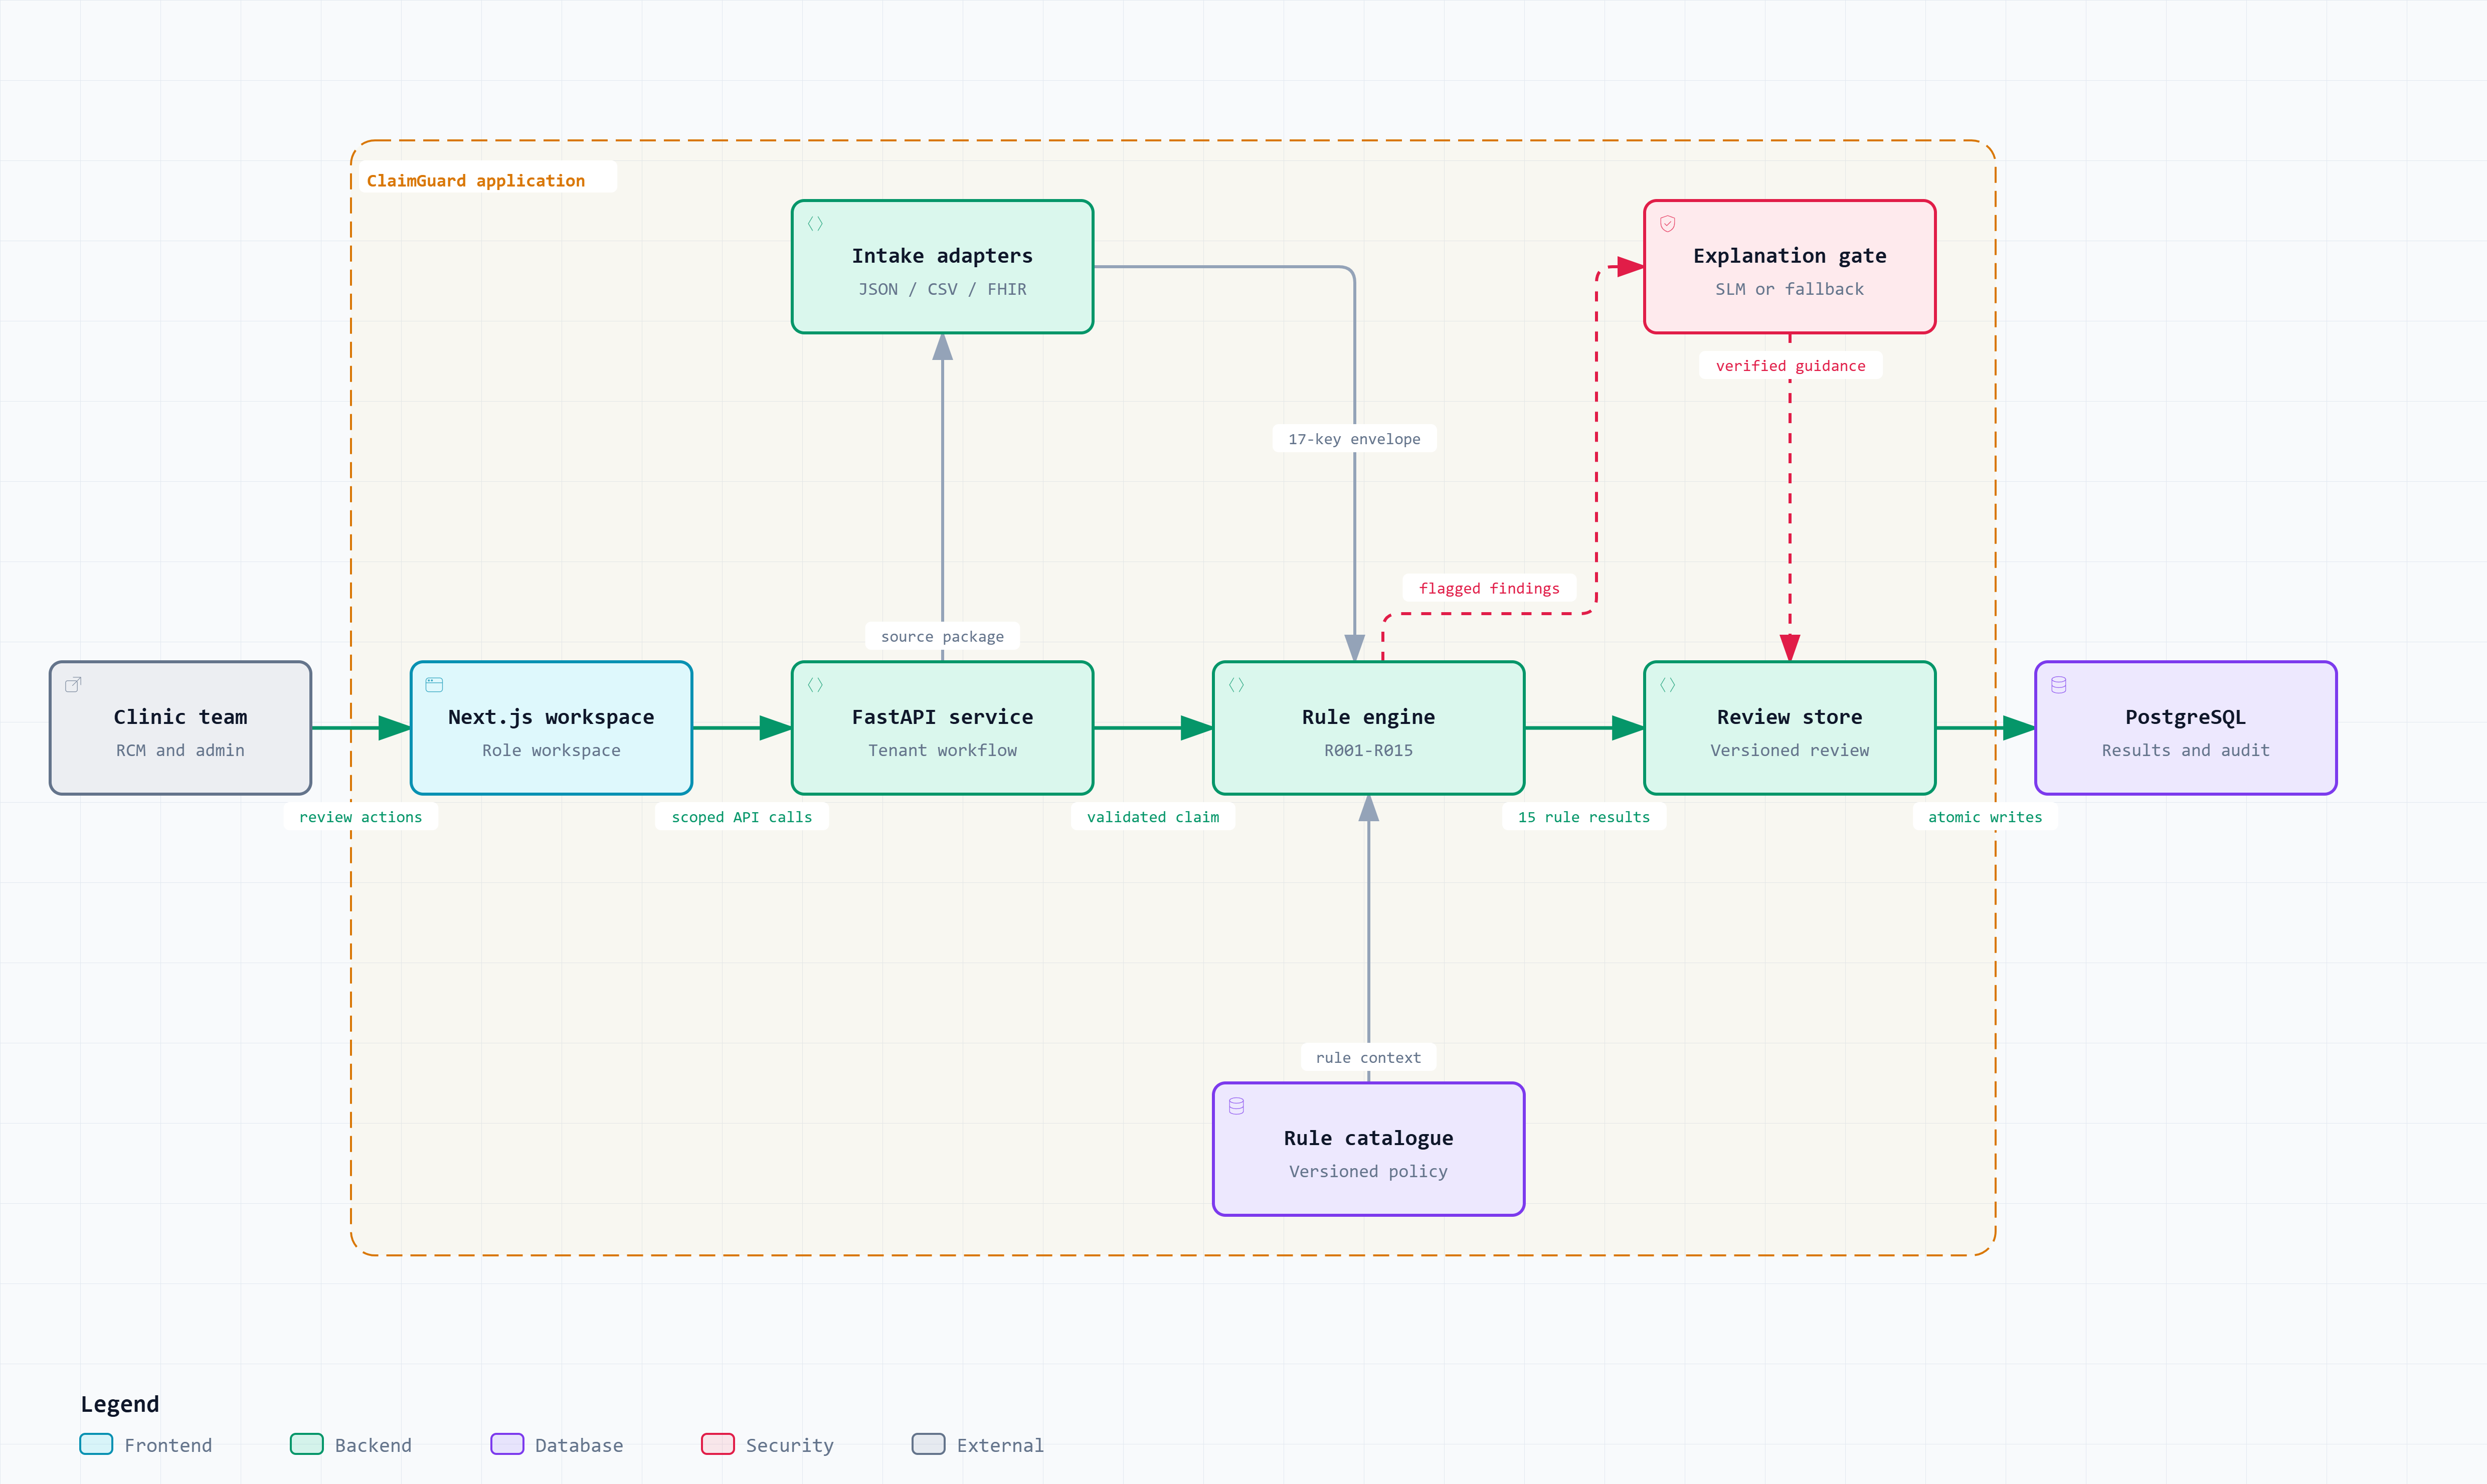
\includegraphics[width=.97\linewidth,height=124mm,keepaspectratio]{assets/system-architecture.png}
\end{center}
\vspace{-2mm}
\begin{minipage}[t]{.49\linewidth}
  \textbf{\color{navy}Who acts and where}\quad Clinic reviewers and admins work in the Next.js interface. It calls the FastAPI service, which applies authentication and clinic scope before reading or changing claim state. The reviewer never edits the rule result directly.
\end{minipage}\hfill
\begin{minipage}[t]{.49\linewidth}
  \textbf{\color{navy}What is authoritative}\quad The rule catalogue and deterministic engine produce the reproducible checks. The review store versions claims, runs, findings, explanations, and decisions in PostgreSQL. An explanation gate can add checked wording; it is not the adjudicator.
\end{minipage}
\newpage

\eyebrow{02 / one claim, end to end}
\claimtitle{Data flow from source to audit}
\vspace{1mm}
{\color{slate}Read this left to right. Green is the primary claim path, red is a guarded policy or evidence path, and grey carries human or versioning actions.}
\vspace{2mm}
\begin{center}
  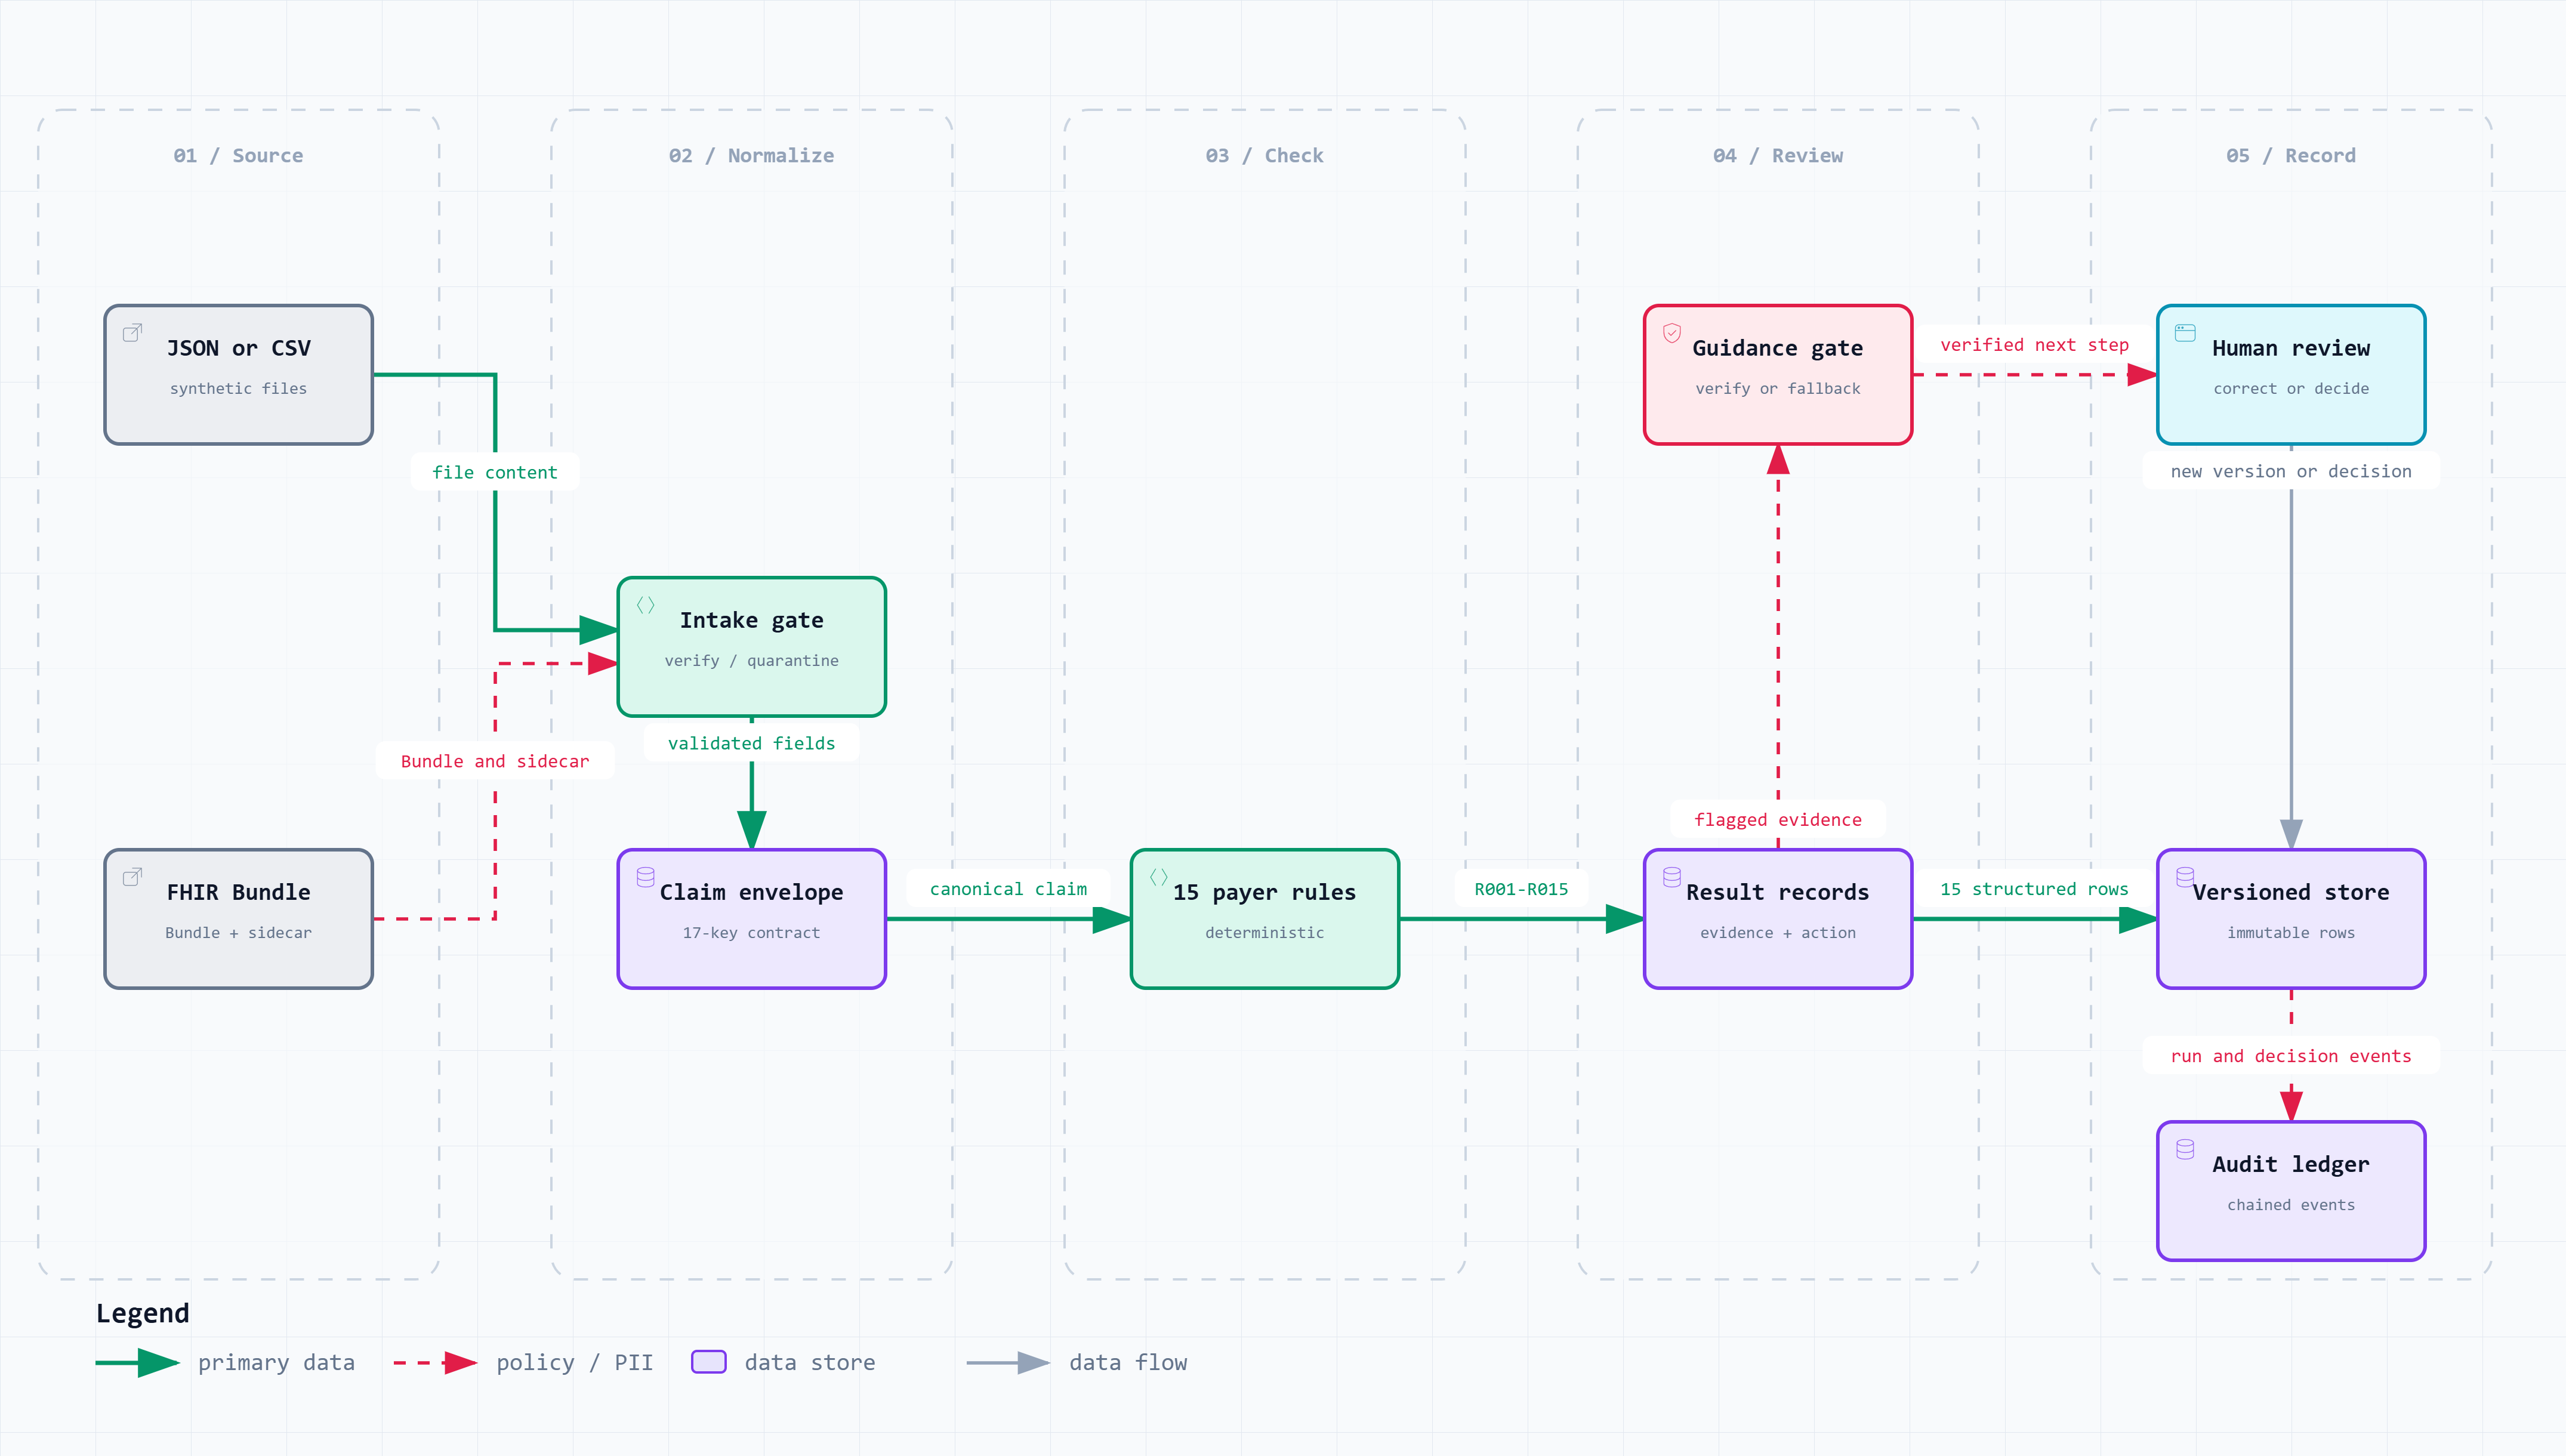
\includegraphics[width=.985\linewidth,height=122mm,keepaspectratio]{assets/claim-data-flow.png}
\end{center}
\vspace{-1mm}
\begin{minipage}[t]{.49\linewidth}
  \textbf{\color{navy}1. Normalize, then check.}\quad A synthetic JSON envelope or supported CSV package passes the intake gate. A FHIR R4 Bundle is supported only with the verified full sidecar needed to fill the scoring contract. Accepted content becomes the same 17-key internal envelope. One claim then produces one result for every rule, R001 through R015.
\end{minipage}\hfill
\begin{minipage}[t]{.49\linewidth}
  \textbf{\color{navy}2. Explain, review, record.}\quad Each result retains its rule identity, evidence and corrective action. When AI wording is requested, a verifier checks it against the finding; unsafe or unsupported wording falls back to deterministic guidance. Corrections create a new claim version and run. Decisions and run events join a hash-chained audit trail.
\end{minipage}
\newpage

\eyebrow{03 / first-submission requirements}
\claimtitle{What the four required parts mean in ClaimGuard}
\vspace{3mm}
\begin{tabularx}{\linewidth}{>{\RaggedRight\arraybackslash}p{.245\linewidth} >{\RaggedRight\arraybackslash}X >{\RaggedRight\arraybackslash}p{.255\linewidth}}
\rowcolor{pale}\textbf{\color{navy}Requirement} & \textbf{\color{navy}Implemented path} & \textbf{\color{navy}Visible artifact}\tabularnewline\hline
\textbf{Data ingestion and normalization}\newline 15 points & Synthetic structured JSON, supported CSV package files, and FHIR R4 Bundle with a required verified sidecar are checked and mapped into the 17-key claim envelope. The scored contract carries patient, coverage, provider, diagnosis and line-item information. & Intake job and normalized claim preview in the workspace; source type, validation and quarantine feedback.\\\hline
\textbf{Deterministic and AI rule engine}\newline 15 points & The versioned fictional payer catalogue defines 15 checks, R001--R015. The deterministic engine generates exactly 15 records per accepted claim. AI assistance is bounded to explanation and correction guidance, not authoritative rule evaluation. & Reproducible run, rule-linked findings and versioned rule context.\\\hline
\textbf{Explainability and structured output}\newline 10 points & Result records carry Claim ID, Rule ID, linked evidence, severity, suggested action and confidence representation. The interface presents the issue beside its next step. Deterministic confidence is not presented as a probability. & Machine-readable results and reviewer-facing guidance tied to the same rule and evidence.\\\hline
\textbf{Audit log engine}\newline 10 points & Runs, finding outputs, explanation provenance and decisions are persisted with version links. Chained run and decision events detect later alteration in the event sequence. & Audit or activity views, version history, and an integrity check for the chained events.\\\hline
\end{tabularx}
\vspace{5mm}
\callout{Important boundary}{The current audit design is tamper-evident for recorded run and decision events. It is not a claim that every UI click or every rejected upload has an immutable audit event. FHIR without a verified sidecar is not a complete direct intake route, and Encounter is not yet retained in the scoring envelope. These are open ingestion and audit gaps.}
\vspace{4mm}
\smalltitle{Why the order matters}
The first gate establishes a consistent claim shape. The engine then evaluates that shape using a fixed rule version. Only after a finding exists does the explanation layer help the reviewer understand it. This ordering makes the result replayable and prevents persuasive text from becoming an untraceable decision.
\newpage

\eyebrow{04 / design rationale and direction}
\claimtitle{Decisions that keep the workflow trustworthy}
\vspace{4mm}
\begin{minipage}[t]{.48\linewidth}
  \smalltitle{A narrow, stable contract}
  Multiple source formats converge on one 17-key envelope. The engine therefore evaluates one predictable structure, while adapters absorb format differences. Invalid or incomplete packages stop at intake rather than receiving invented values.\par\medskip
  \smalltitle{Rules before language generation}
  The fictional payer rulebook is explicit and versioned. Exactly one result per rule gives completeness and repeatability. Model-generated prose is checked against rule evidence and rejected when it adds unsupported facts. The human reviewer remains responsible for a correction or decision.\par\medskip
  \smalltitle{Versioning before overwriting}
  A correction starts a new claim version and validation run, preserving the earlier state. This is essential for explaining what changed and why a later result differs from the first.
\end{minipage}\hfill
\begin{minipage}[t]{.48\linewidth}
  \smalltitle{Clinic isolation at the service boundary}
  Role and tenant checks are applied by the API and storage access path. The interface can guide the right workspace, but it is not relied on as the security boundary. Technical operations are separated from claim content access.\par\medskip
  \smalltitle{Next work already under way}
  \begin{itemize}
    \item Evaluate small language models on evidence fidelity and useful correction guidance before selecting one for default use.
    \item Broaden FHIR mapping and prototype document-to-draft extraction using synthetic clinical documents, with human confirmation before scoring.
    \item Extend audit coverage around intake failures and administrative actions, then verify the chain under tampering and replay tests.
    \item Explore JEV only at a tightly specified advisory step, with scoped inputs, traceable outputs and no authority to alter payer-rule decisions.
  \end{itemize}
\end{minipage}
\vfill

\begin{tikzpicture}
  \fill[navy] (0,0) rectangle (26.1,1.65);
  \node[anchor=west,text=white,font=\large\bfseries] at (.55,.98) {The outcome};
  \node[anchor=west,text=mint,font=\normalsize] at (.55,.42) {A reviewer can trace a finding back to its source, rule, evidence, version and recorded action.};
\end{tikzpicture}
\end{document}
